\documentclass[11pt,a4paper]{article}
\usepackage{fontspec}
\setmainfont{TeX Gyre Pagella}
\newfontfamily\headfont{Inter}[UprightFont=*-ExtraBold,BoldFont=*-ExtraBold,Extension=.otf,Path=/usr/share/fonts/opentype/inter/]
\usepackage[a4paper,margin=2.3cm]{geometry}
\usepackage{graphicx,booktabs,float,caption,array,xcolor,longtable}
\usepackage{xurl}
\usepackage[hidelinks]{hyperref}
\usepackage{titlesec}
\usepackage[round]{natbib}
\usepackage{setspace}
\setstretch{1.05}
\renewcommand{\topfraction}{0.9}
\renewcommand{\bottomfraction}{0.8}
\renewcommand{\textfraction}{0.1}
\renewcommand{\floatpagefraction}{0.75}
\setlength{\parindent}{0pt}
\setlength{\parskip}{0.55em}
\titleformat{\section}{\headfont\Large}{\thesection}{0.8em}{}
\titleformat{\subsection}{\headfont\large}{\thesubsection}{0.8em}{}
\captionsetup{font=small,labelfont=bf}
\urlstyle{same}
\hypersetup{pdftitle={Where Every Film Director Is From},pdfauthor={Tristan Hotham}}

\begin{document}
\begin{center}
{\Large\bfseries Where Every Film Director Is From\par}
\vspace{0.4em}
{\large The birthplaces of 43,619 film directors in Wikidata,\\by city, country, debut decade, gender and country of work\par}
\vspace{1.2em}
{\large Tristan Hotham\par}
\vspace{0.3em}
{\small Independent researcher\\
ORCID: 0000-0003-4931-9349\\
DOI: \href{https://doi.org/10.5281/zenodo.23847840}{https://doi.org/10.5281/zenodo.23847840}\par}
\vspace{0.8em}
2026
\end{center}

\begin{quote}
\small
\begin{center}\textbf{Abstract}\end{center}
Where are film directors born, and how has that changed? I use Wikidata, the open knowledge base behind Wikipedia, to map the birthplaces of everyone it records as the director of a film. Of 78,729 directors, 43,619 (55\%) have a birth country and 41,753 a birthplace with coordinates, in 188 present-day countries. The United States accounts for 17\% of directors with a birth country and 38\% of notable ones (those with 20 or more sitelinks). Grouping birthplaces into city areas, New York (1,469) and Paris (1,368) lead; per head of present population, Prague (45.1 per 100,000) and Copenhagen (37.6). By debut decade, the share born in Europe or North America falls from 83\% for directors who debuted by the 1950s to 67\% for those who debuted since 2000, while Asia's rises from 12\% to 23\%. 15\% of directors made their films mainly in a country other than their birth country; the largest flow is from the United Kingdom to the United States (416 directors). Women are 3.1\% of directors who debuted in the 1920s and 32\% of those who debuted in the 2020s. Coverage is very uneven: a birthplace is recorded for 99.5\% of notable directors but 25\% of those with at most one sitelink, and for 33\% of directors whose films are mainly Nigerian. The atlas maps the open record of film, not every film-maker.

\textbf{Keywords:} film directors; cinema history; birthplaces; migration; gender; Wikidata; open data; mapping
\end{quote}

\section{Introduction}
Film history is usually told through national cinemas, studios and movements. Yet film-making has always been mobile: Hollywood was built in part by directors from Europe \citep{petrie}, and new industries in India, South Korea, Iran and Nigeria \citep{haynes} have produced directors in large numbers. A simple question cuts across these stories: where were the people who directed films born?

Wikidata \citep{wikidata} offers a way to ask it at scale. It records tens of thousands of film directors, many with a place and date of birth, and links them to films with release dates and countries of origin. Studies of notable people's birth and death places have shown how much structure such data hold, and how much they reflect the biases of the sources \citep{schich}. This paper maps directors' birthplaces by city, country and debut decade, compares birth country with the country of a director's films, and tracks the share of women. It pairs the analysis with an interactive atlas (\url{https://maps.tristanhotham.com/director-birthplaces/}).

The contribution is descriptive. Wikidata is not a census of film-makers. Its coverage depends on which film databases have been imported and which people have Wikipedia articles, and its records of gender follow those of Wikipedia, where women are known to be under-represented \citep{wagner}. I report coverage alongside every result.

\section{Data}
\textbf{Directors.} A query through the QLever SPARQL endpoint \citep{qlever}, retrieved in 2026, returned every item that is the director (P57) of at least one item that is an instance of film (Q11424), with its English label, place of birth (P19), that place's coordinates (P625) and country (P17), date of birth (P569), gender (P21), number of sitelinks and number of films directed. Because each combination of values is a row, the result has 82,886 rows; after dropping 91 rows for directors recorded only as unknown values, it covers 78,729 directors. The query asks only for directors of films, so it includes actors, musicians and artists who directed a single film and a few bands credited with concert films. 978 directors have no English label in the extract.

\textbf{Films.} A second query returned 282,877 director credits on 264,652 film items, with each film's publication date (P577) and country of origin (P495). One line of the result was missing a line break and was repaired.

\textbf{Geography.} Natural Earth \citep{naturalearth} countries (1:10m for assigning points, 1:50m for display) and populated places, with population estimates. All Wikidata content is CC0 and Natural Earth is public domain.

\begin{table}[tbp]\centering\small\caption{From query to data.}\label{tab:pipe}\begin{tabular}{p{10cm}r}\toprule Step & Directors\\\midrule
Rows returned by the director query & 82,886\\
Directors (after dropping unknown values) & 78,729\\
\quad with a birthplace & 43,632\\
\quad with a birth country & 43,619\\
\quad with a birthplace point (on the map) & 41,753\\
\quad\quad of which in a city area of a million or more & 22,896\\
\quad with a year of birth & 52,615\\
\quad with a recorded gender & 71,115\\
\quad with a dated film (debut decade) & 74,541\\
\quad with a main film country & 76,520\\
\quad notable (20+ sitelinks) & 3,835\\
Film items linked to these directors & 264,652\\
\bottomrule\end{tabular}\end{table}

\section{Methods}
\subsection{Birthplaces and birth countries}
A director's birthplace is the first place of birth in the result (367 directors have more than one) and its point is that place's coordinates. 1,770 birthplaces are themselves countries (for example `United States'); these give a country but no point. The birth country is the present-day Natural Earth country that the point falls in, else the birthplace's Wikidata country matched to Natural Earth by Wikidata identifier. Where both are known they agree for 99\% of 43,349 directors; most differences are historical states recorded as the country of a place.

\subsection{City areas and per-head rates}
Wikidata often records a district (Brooklyn, a Paris arrondissement, Neuilly-sur-Seine) rather than a city. To compare cities I assign each birthplace point to the nearest Natural Earth populated place of one million people or more within 30 km, merging any such place that lies within 30 km of a larger one (Howrah into Kolkata, Yokohama into Tokyo). 55\% of points fall in one of 413 city areas. Per-head rates divide by Natural Earth's present-day metropolitan population, and are shown only for cities with 50 or more directors. They are a rough guide: most directors were born decades ago, when cities were smaller and in different proportion to each other.

\subsection{Debut decade and country of work}
A director's debut year is the earliest publication year (1880 to 2026) of any film credited to them; 95\% have one. Debut decades before 1910 are pooled. A director's main film country is the country of origin with the largest share of their films, each film's weight split equally between its countries of origin. Films credited to former states are assigned to a principal present-day successor, and when testing whether a director worked abroad a former state counts for all its successors (the Soviet Union for Russia, Ukraine, Georgia and the others; Yugoslavia, Czechoslovakia, the German states and British India likewise), so that a Ukrainian-born Soviet director is not counted as a migrant. A director worked abroad if their birth country is not their main film country, which needs both a birth country and a film with a country of origin (42,950 directors).

\subsection{Gender and notability}
Women and trans women are counted as women and men and trans men as men; 63 directors have another gender recorded. Shares are among directors with a recorded gender (90\%). Notable directors are those with 20 or more sitelinks (3,835 directors, 5\%), a measure of attention on Wikipedia and its sister projects, not of artistic standing.

\section{Results}
\subsection{The map}
Figure~\ref{fig:map} shows all 41,753 birthplace points in hexagons. They are densest in Europe, the north-eastern United States, California, India, Japan and Korea, and sparse across Africa, Central Asia and much of South America. Europe accounts for 51\% of directors with a birth country, North America 21\%, Asia 20\%, South America 4\%, Africa 2.8\% and Oceania 1.2\%. The maps of women and of notable directors (Figure~\ref{fig:wn}) have the same broad shape, with notable directors concentrated even more strongly in the United States.

\begin{figure}[tbp]\centering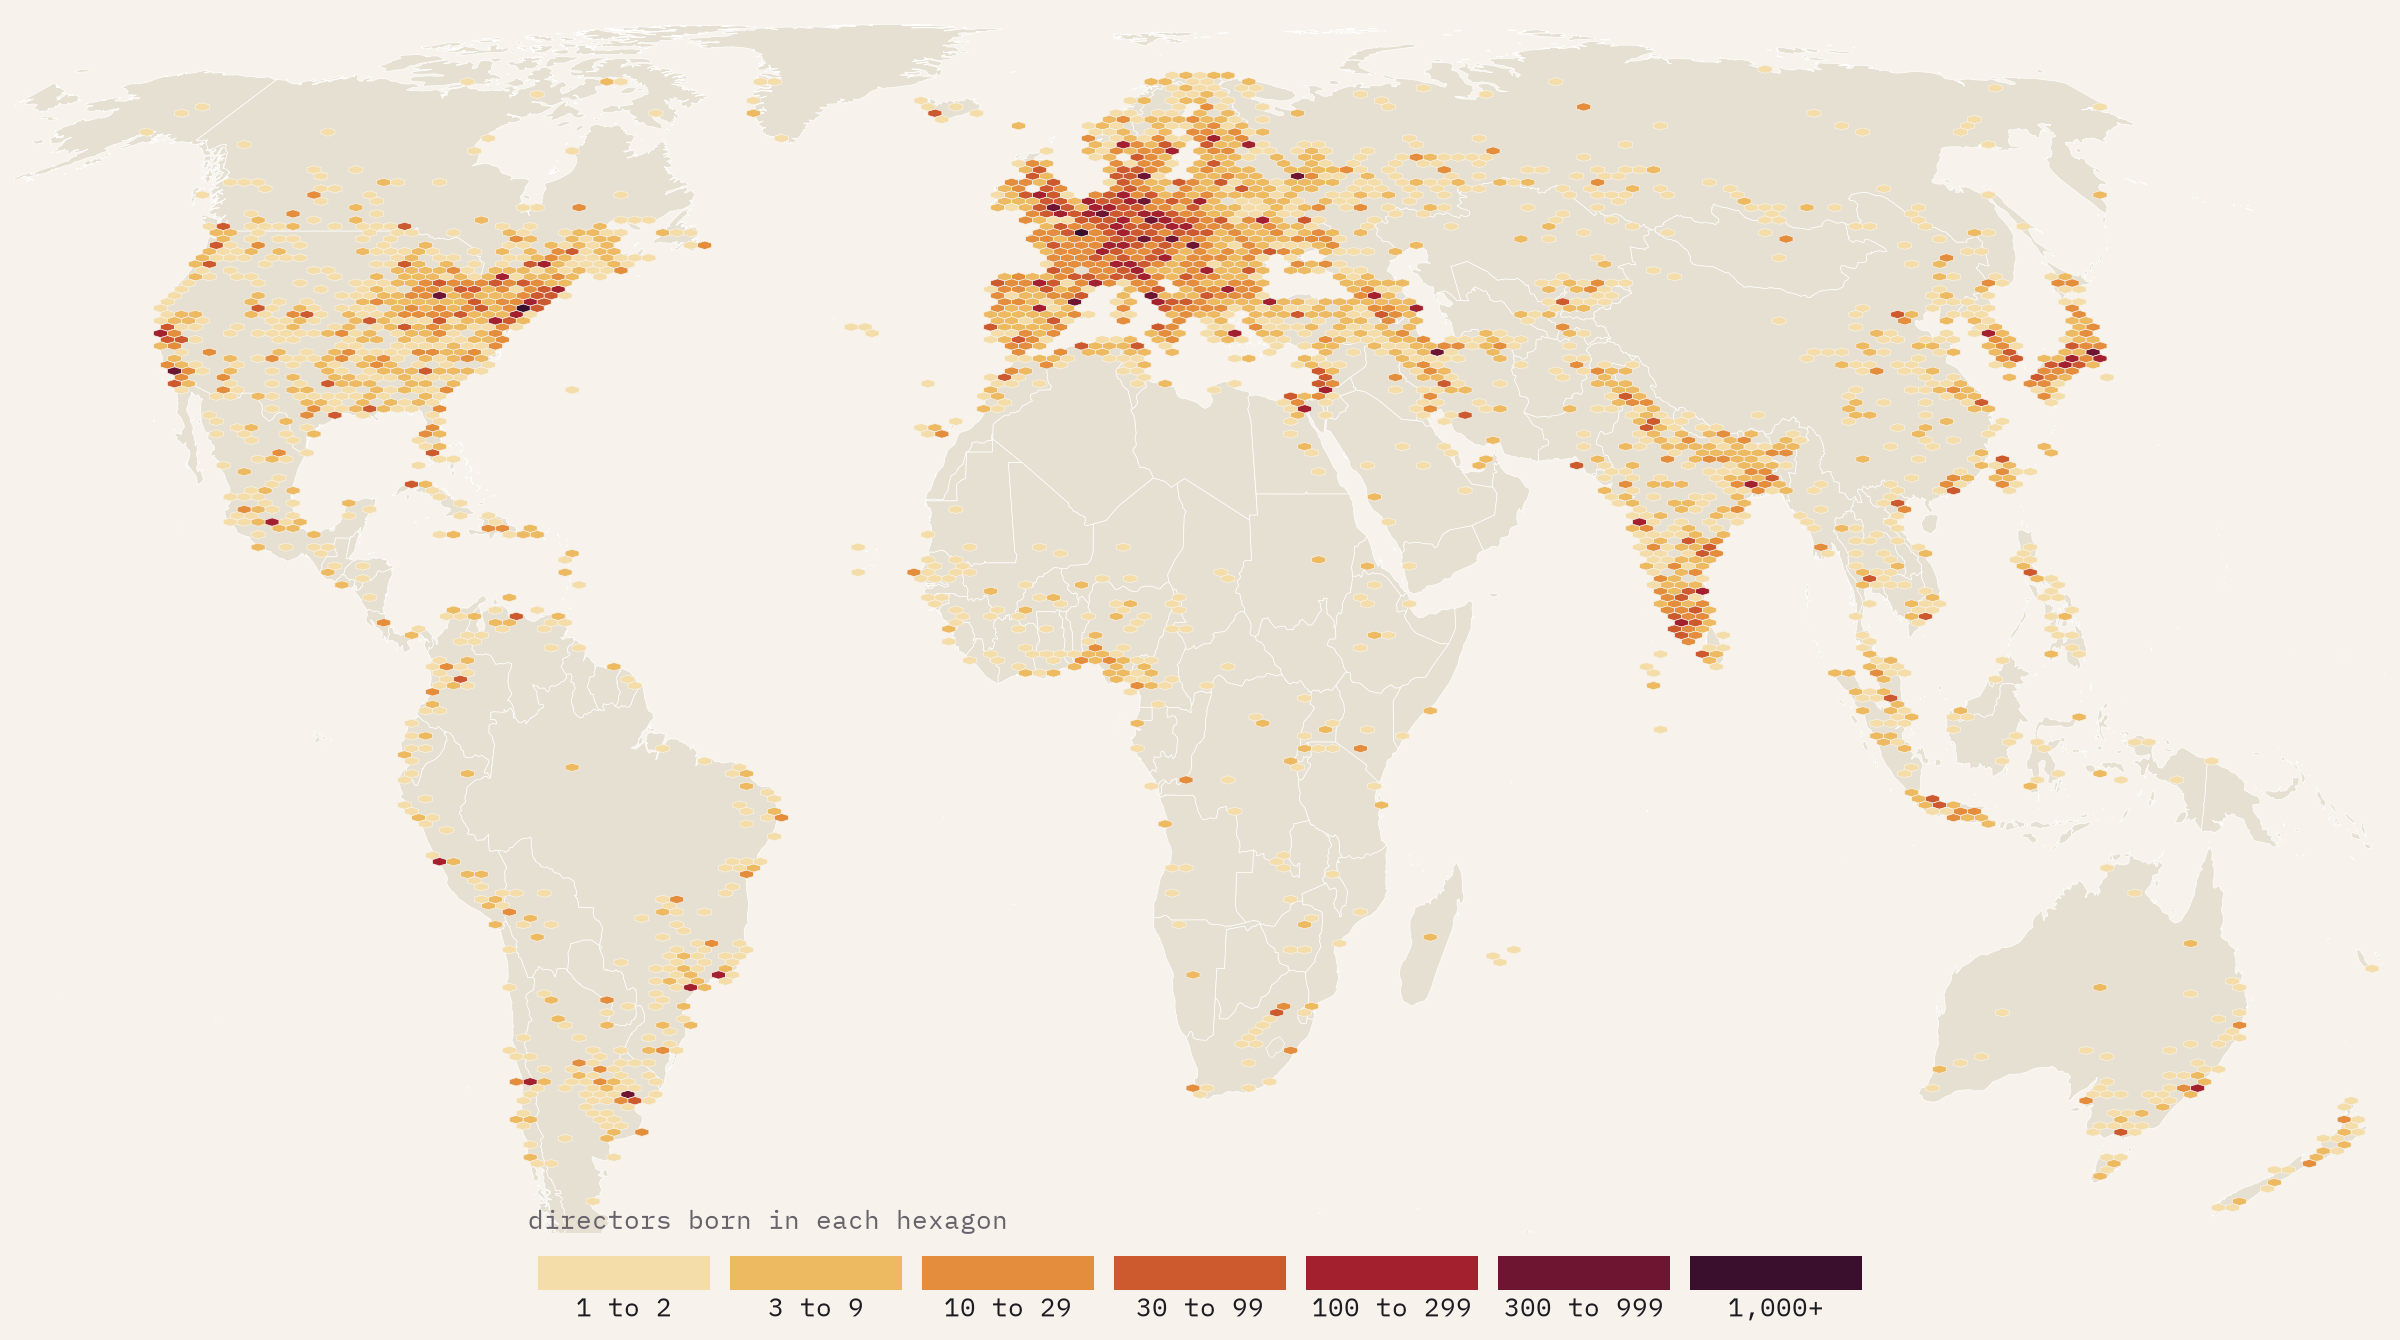
\includegraphics[width=\textwidth]{f_map.png}
\caption{Birthplaces of 41,753 film directors in Wikidata, counted in hexagons (Equal Earth projection).}\label{fig:map}\end{figure}

\begin{figure}[tbp]\centering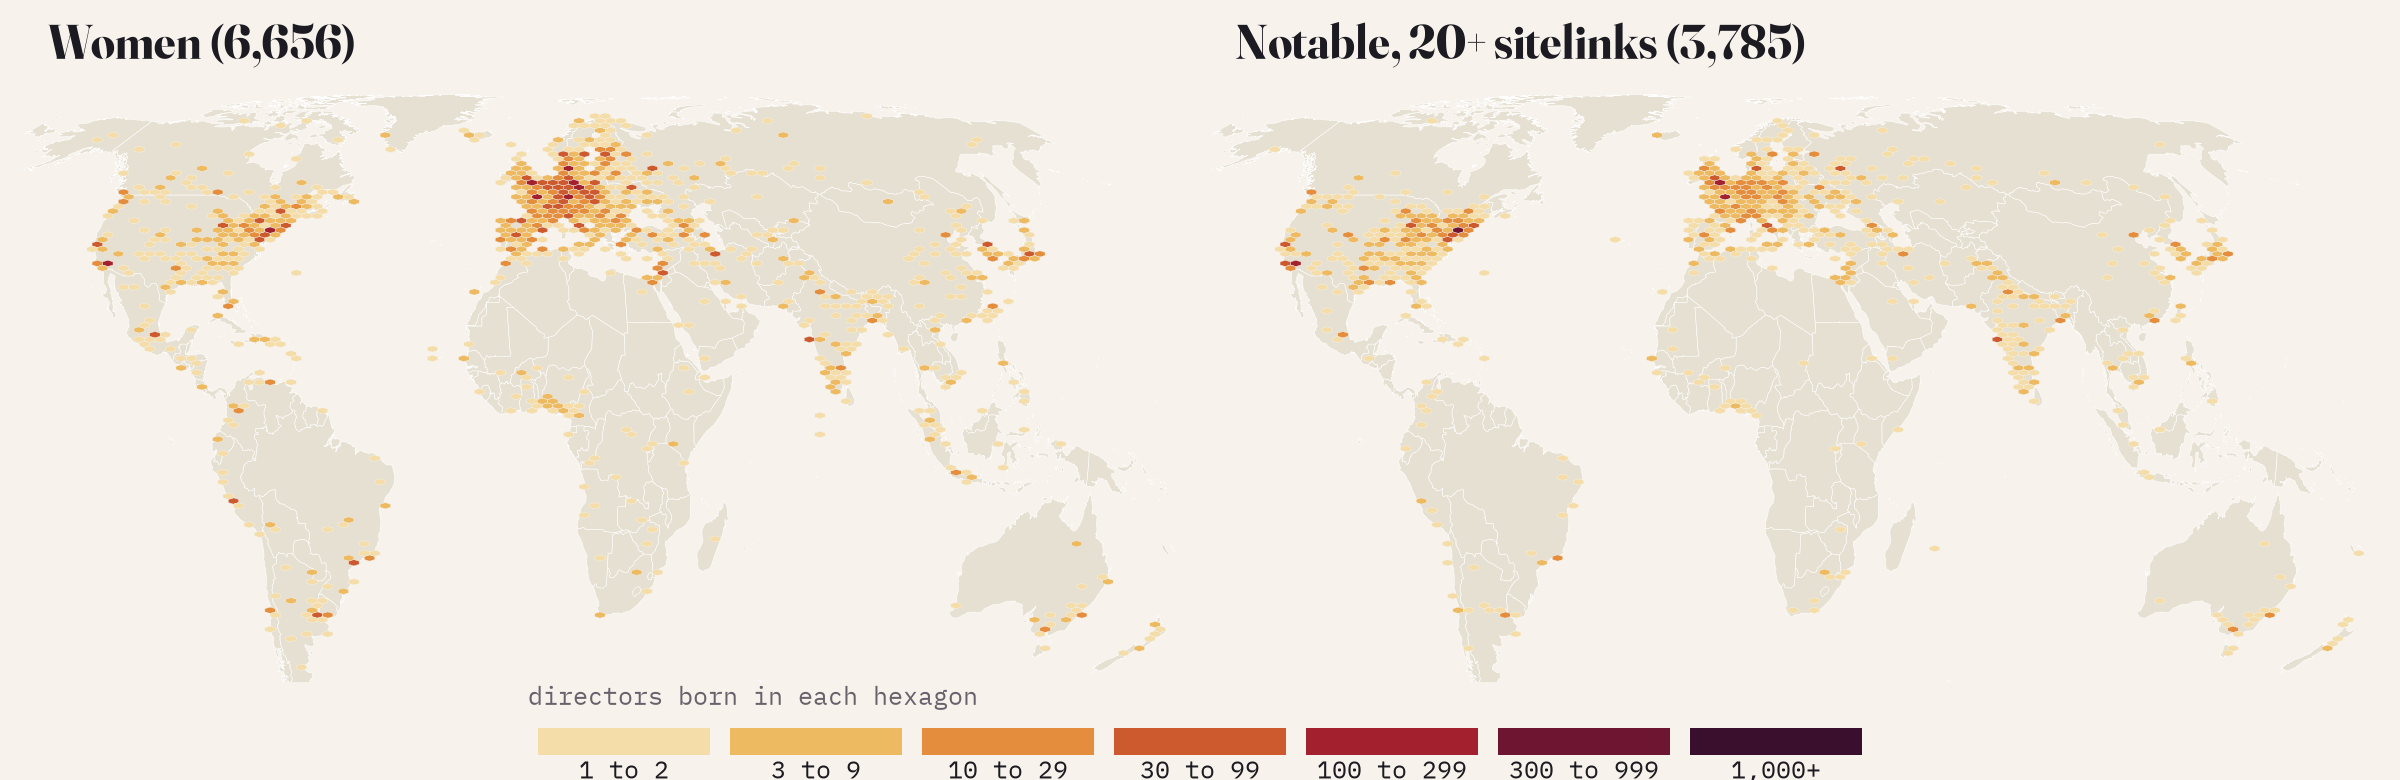
\includegraphics[width=\textwidth]{f_women_notable_maps.png}
\caption{Birthplaces of women directors (left) and of notable directors, with 20 or more sitelinks (right).}\label{fig:wn}\end{figure}

\subsection{Cities}
As recorded in Wikidata, the birthplace with most directors is New York City (847), then Rome (626), London (508) and Prague (486). Grouped into city areas (Figure~\ref{fig:cities}, Table~\ref{tab:cities}), New York (1,469) and Paris (1,368) lead by a wide margin; Paris gains most from grouping, because many Parisians are recorded by arrondissement. The ten largest city areas account for 17\% of all birthplace points. Per head of present population the leaders are Prague, Copenhagen, Munich, Stockholm and Rome, while the largest cities of Asia, Latin America and Africa have very low rates: Tokyo 1.1, Mumbai 1.1 and Kolkata 1.0 per 100,000, against New York's 7.7.

\begin{figure}[tbp]\centering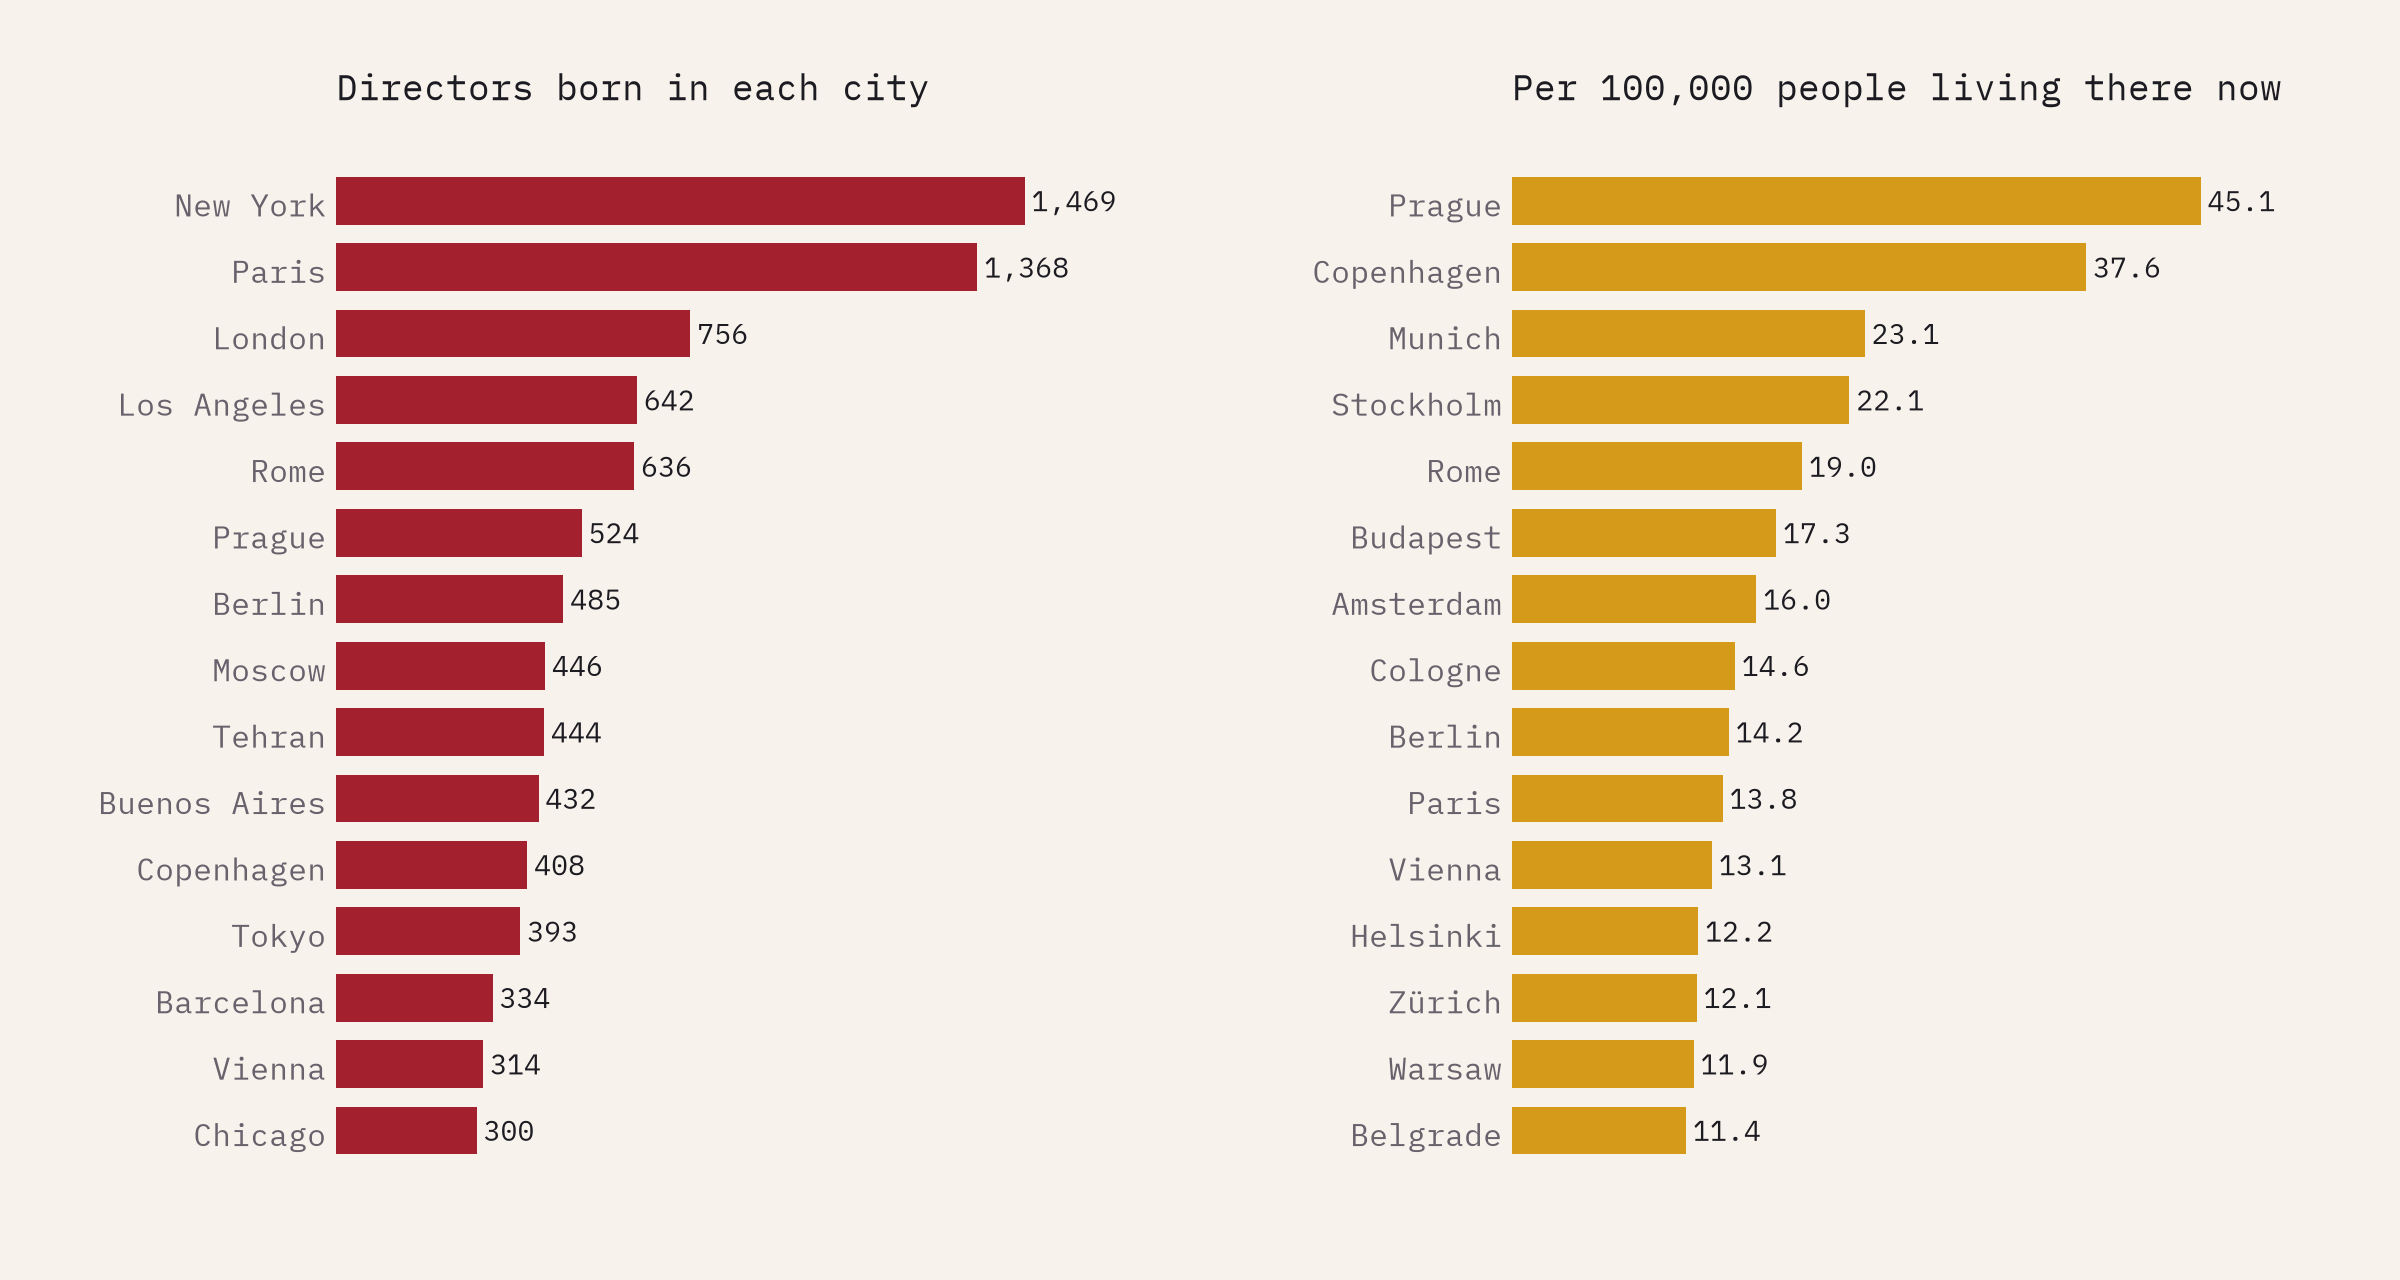
\includegraphics[width=\textwidth]{f_cities.png}
\caption{City areas (birthplaces within 30 km of a city of a million or more) with most directors, and with most per 100,000 present-day residents (cities with 50+ directors).}\label{fig:cities}\end{figure}

\begin{table}[tbp]\centering\small\caption{City areas: most directors (with notable directors and the share of women), and most directors per 100,000 present-day residents.}\label{tab:cities}\setlength{\tabcolsep}{5pt}\begin{tabular}{lrrr@{\hspace{18pt}}lrr}\toprule City & Directors & Notable & Women & City & Directors & Per 100,000\\\midrule
New York & 1,469 & 321 & 13\% & Prague & 524 & 45.1\\
Paris & 1,368 & 205 & 19\% & Copenhagen & 408 & 37.6\\
London & 756 & 127 & 13\% & Munich & 294 & 23.1\\
Los Angeles & 642 & 142 & 20\% & Stockholm & 279 & 22.1\\
Rome & 636 & 55 & 10\% & Rome & 636 & 19.0\\
Prague & 524 & 12 & 17\% & Budapest & 291 & 17.3\\
Berlin & 485 & 25 & 24\% & Amsterdam & 165 & 16.0\\
Moscow & 446 & 38 & 15\% & Cologne & 147 & 14.6\\
Tehran & 444 & 15 & 11\% & Berlin & 485 & 14.2\\
Buenos Aires & 432 & 16 & 19\% & Paris & 1,368 & 13.8\\
Copenhagen & 408 & 25 & 21\% & Vienna & 314 & 13.1\\
Tokyo & 393 & 22 & 9\% & Helsinki & 136 & 12.2\\
Barcelona & 334 & 13 & 22\% & Zürich & 134 & 12.1\\
Vienna & 314 & 23 & 13\% & Warsaw & 203 & 11.9\\
Chicago & 300 & 68 & 14\% & Belgrade & 125 & 11.4\\
\bottomrule\end{tabular}\end{table}

\subsection{Countries}
The United States is the birth country of 7,243 directors (17\%), followed by Germany, France, Italy and India (Figure~\ref{fig:countries}, Table~\ref{tab:countries}); the five together account for 41\%. Among notable directors the United States accounts for 38\%, and France and the United Kingdom rise above Germany. Germany, the Czech Republic and Denmark rank higher among all directors than among notable ones, a sign of systematic import of their national film records.

\begin{figure}[tbp]\centering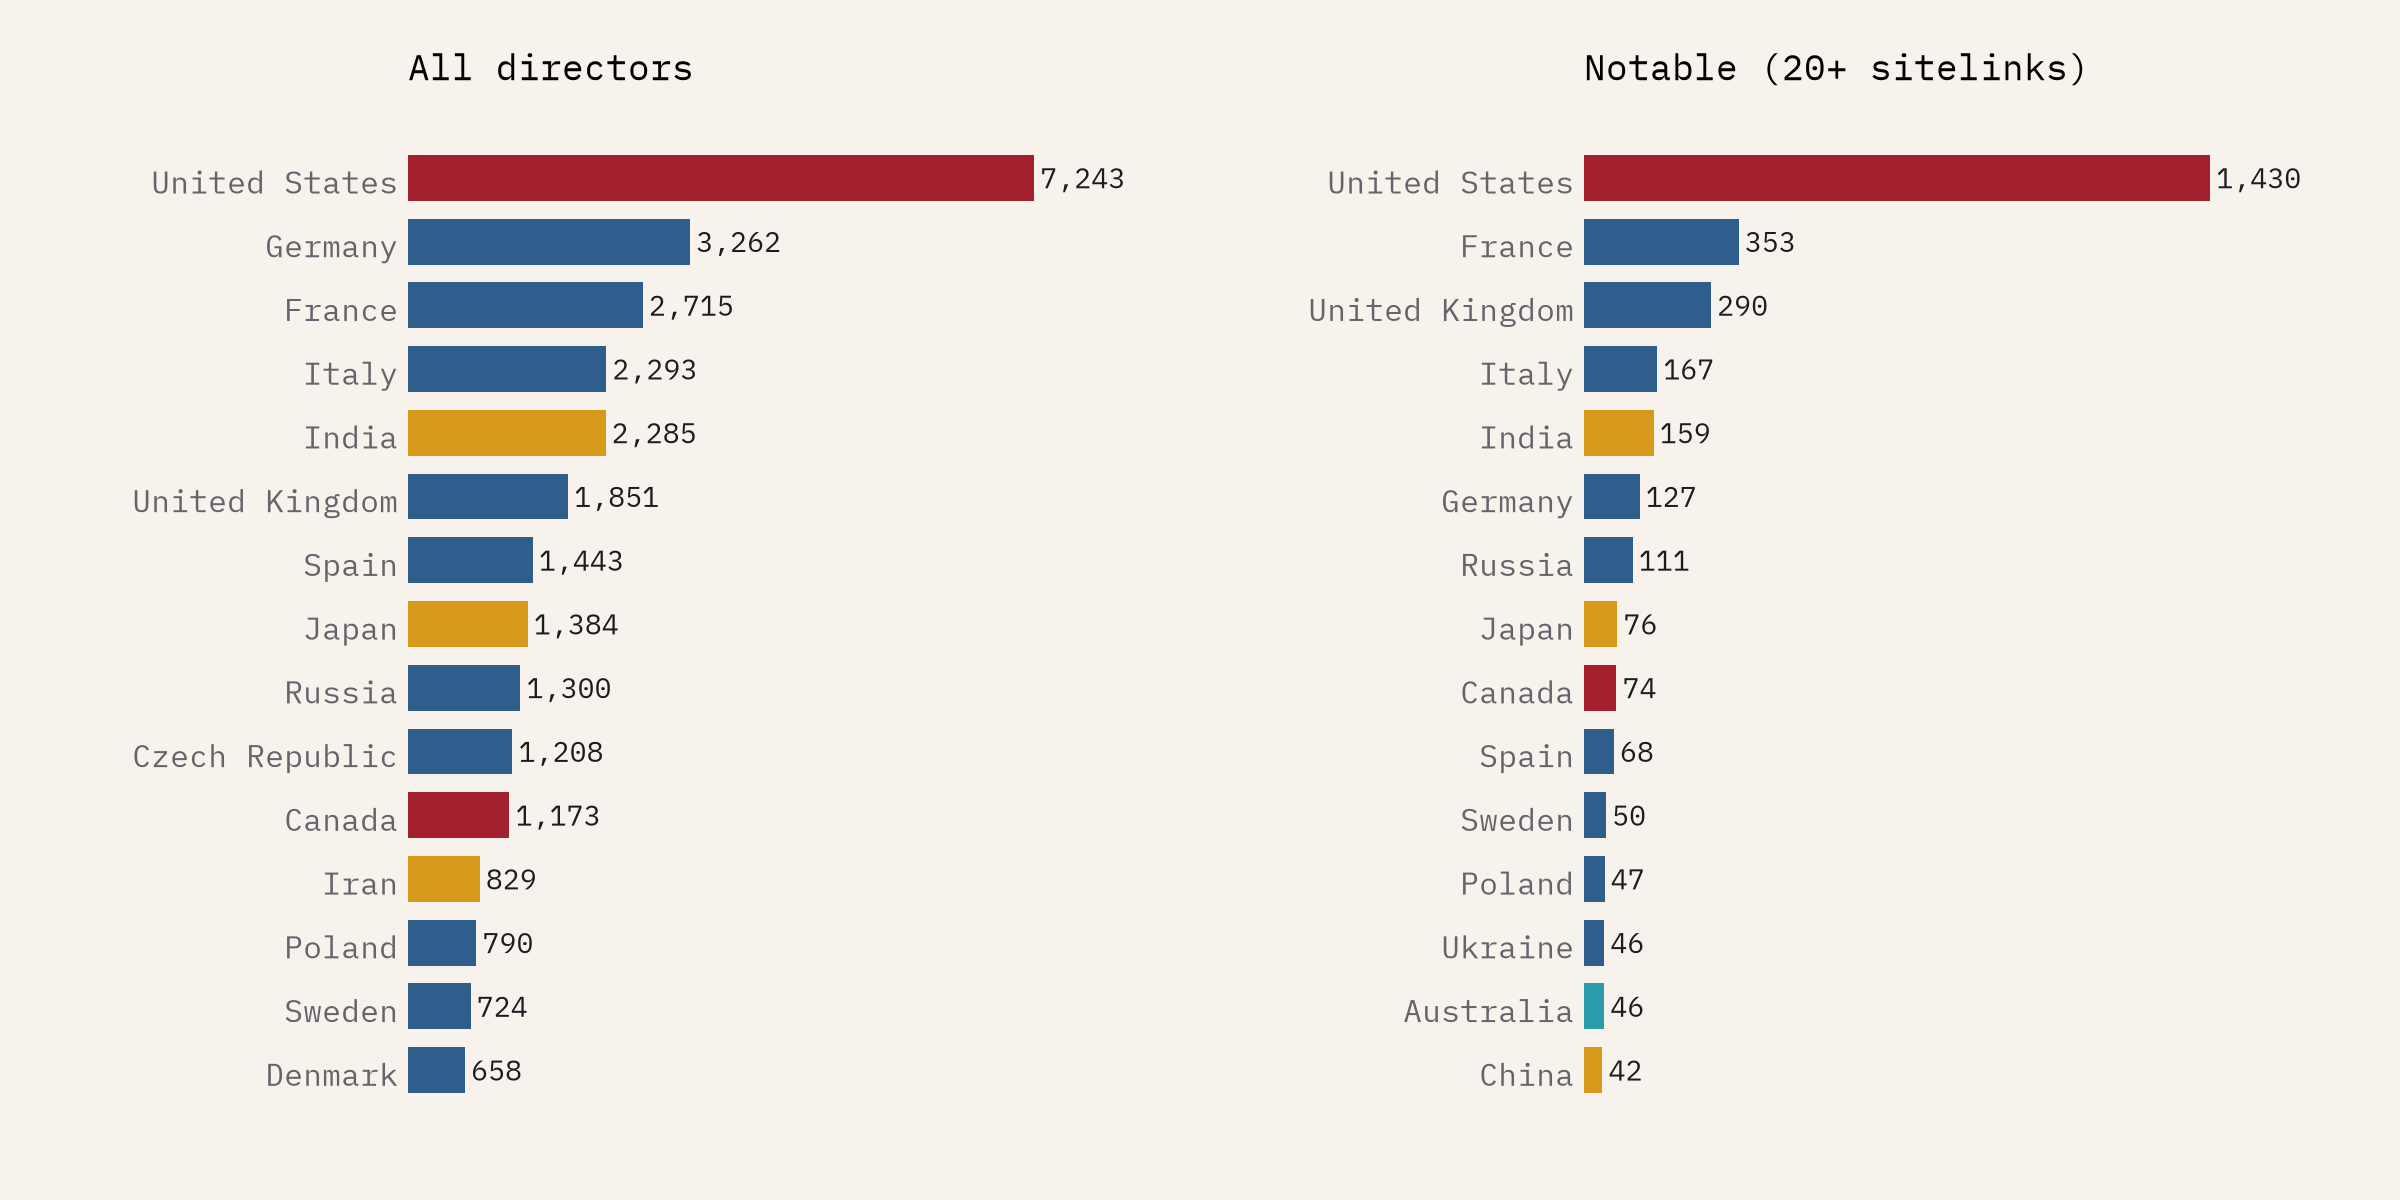
\includegraphics[width=\textwidth]{f_countries.png}
\caption{Directors by country of birth: all directors with a birth country, and notable directors. Colours: continent.}\label{fig:countries}\end{figure}

\begin{table}[tbp]\centering\small\caption{The twenty countries of birth with most directors: share of all directors with a birth country, notable directors, women's share, and directors per million present-day population.}\label{tab:countries}\begin{tabular}{lrrrrr}\toprule Country & Directors & Share & Notable & Women & Per million\\\midrule
United States & 7,243 & 16.6\% & 1,430 & 14.8\% & 22.1\\
Germany & 3,262 & 7.5\% & 127 & 23.3\% & 39.2\\
France & 2,715 & 6.2\% & 353 & 18.5\% & 40.5\\
Italy & 2,293 & 5.3\% & 167 & 9.3\% & 38.0\\
India & 2,285 & 5.2\% & 159 & 8.2\% & 1.7\\
United Kingdom & 1,851 & 4.2\% & 290 & 11.4\% & 27.7\\
Spain & 1,443 & 3.3\% & 68 & 19.4\% & 30.7\\
Japan & 1,384 & 3.2\% & 76 & 8.5\% & 11.0\\
Russia & 1,300 & 3.0\% & 111 & 13.9\% & 9.0\\
Czech Republic & 1,208 & 2.8\% & 34 & 14.6\% & 113.2\\
Canada & 1,173 & 2.7\% & 74 & 26.7\% & 31.2\\
Iran & 829 & 1.9\% & 25 & 9.3\% & 10.0\\
Poland & 790 & 1.8\% & 47 & 16.6\% & 20.8\\
Sweden & 724 & 1.7\% & 50 & 20.9\% & 70.4\\
Denmark & 658 & 1.5\% & 32 & 19.5\% & 113.1\\
Argentina & 615 & 1.4\% & 24 & 17.2\% & 13.7\\
Ukraine & 566 & 1.3\% & 46 & 13.3\% & 12.8\\
Brazil & 562 & 1.3\% & 22 & 16.6\% & 2.7\\
Austria & 553 & 1.3\% & 32 & 17.0\% & 62.3\\
South Korea & 550 & 1.3\% & 34 & 17.3\% & 10.6\\
\bottomrule\end{tabular}\end{table}

\subsection{The shift by debut decade}
Figure~\ref{fig:shift} shows directors' continents of birth by debut decade. Europe accounts for about three fifths of each decade's directors from the 1910s to the 1960s, then falls to around half; North America's share is highest in the 1910s (36.1\%) and lowest in the 1950s and 1960s; Asia grows from 1.6\% in the 1910s to 24.0\% in the 2010s. Among countries (Figure~\ref{fig:rise}), the United States falls from 33.9\% of directors who debuted in the 1910s to 14.9\% in the 2010s, India rises from 3.1\% of those who debuted by the 1950s to 6.0\% since 2000, South Korea from 0.2\% to 1.9\% and Iran from 0.5\% to 1.9\%. Nigeria, home of one of the world's most productive film industries \citep{haynes}, barely registers (0.6\% since 2000), a gap in the record discussed below.

\begin{figure}[tbp]\centering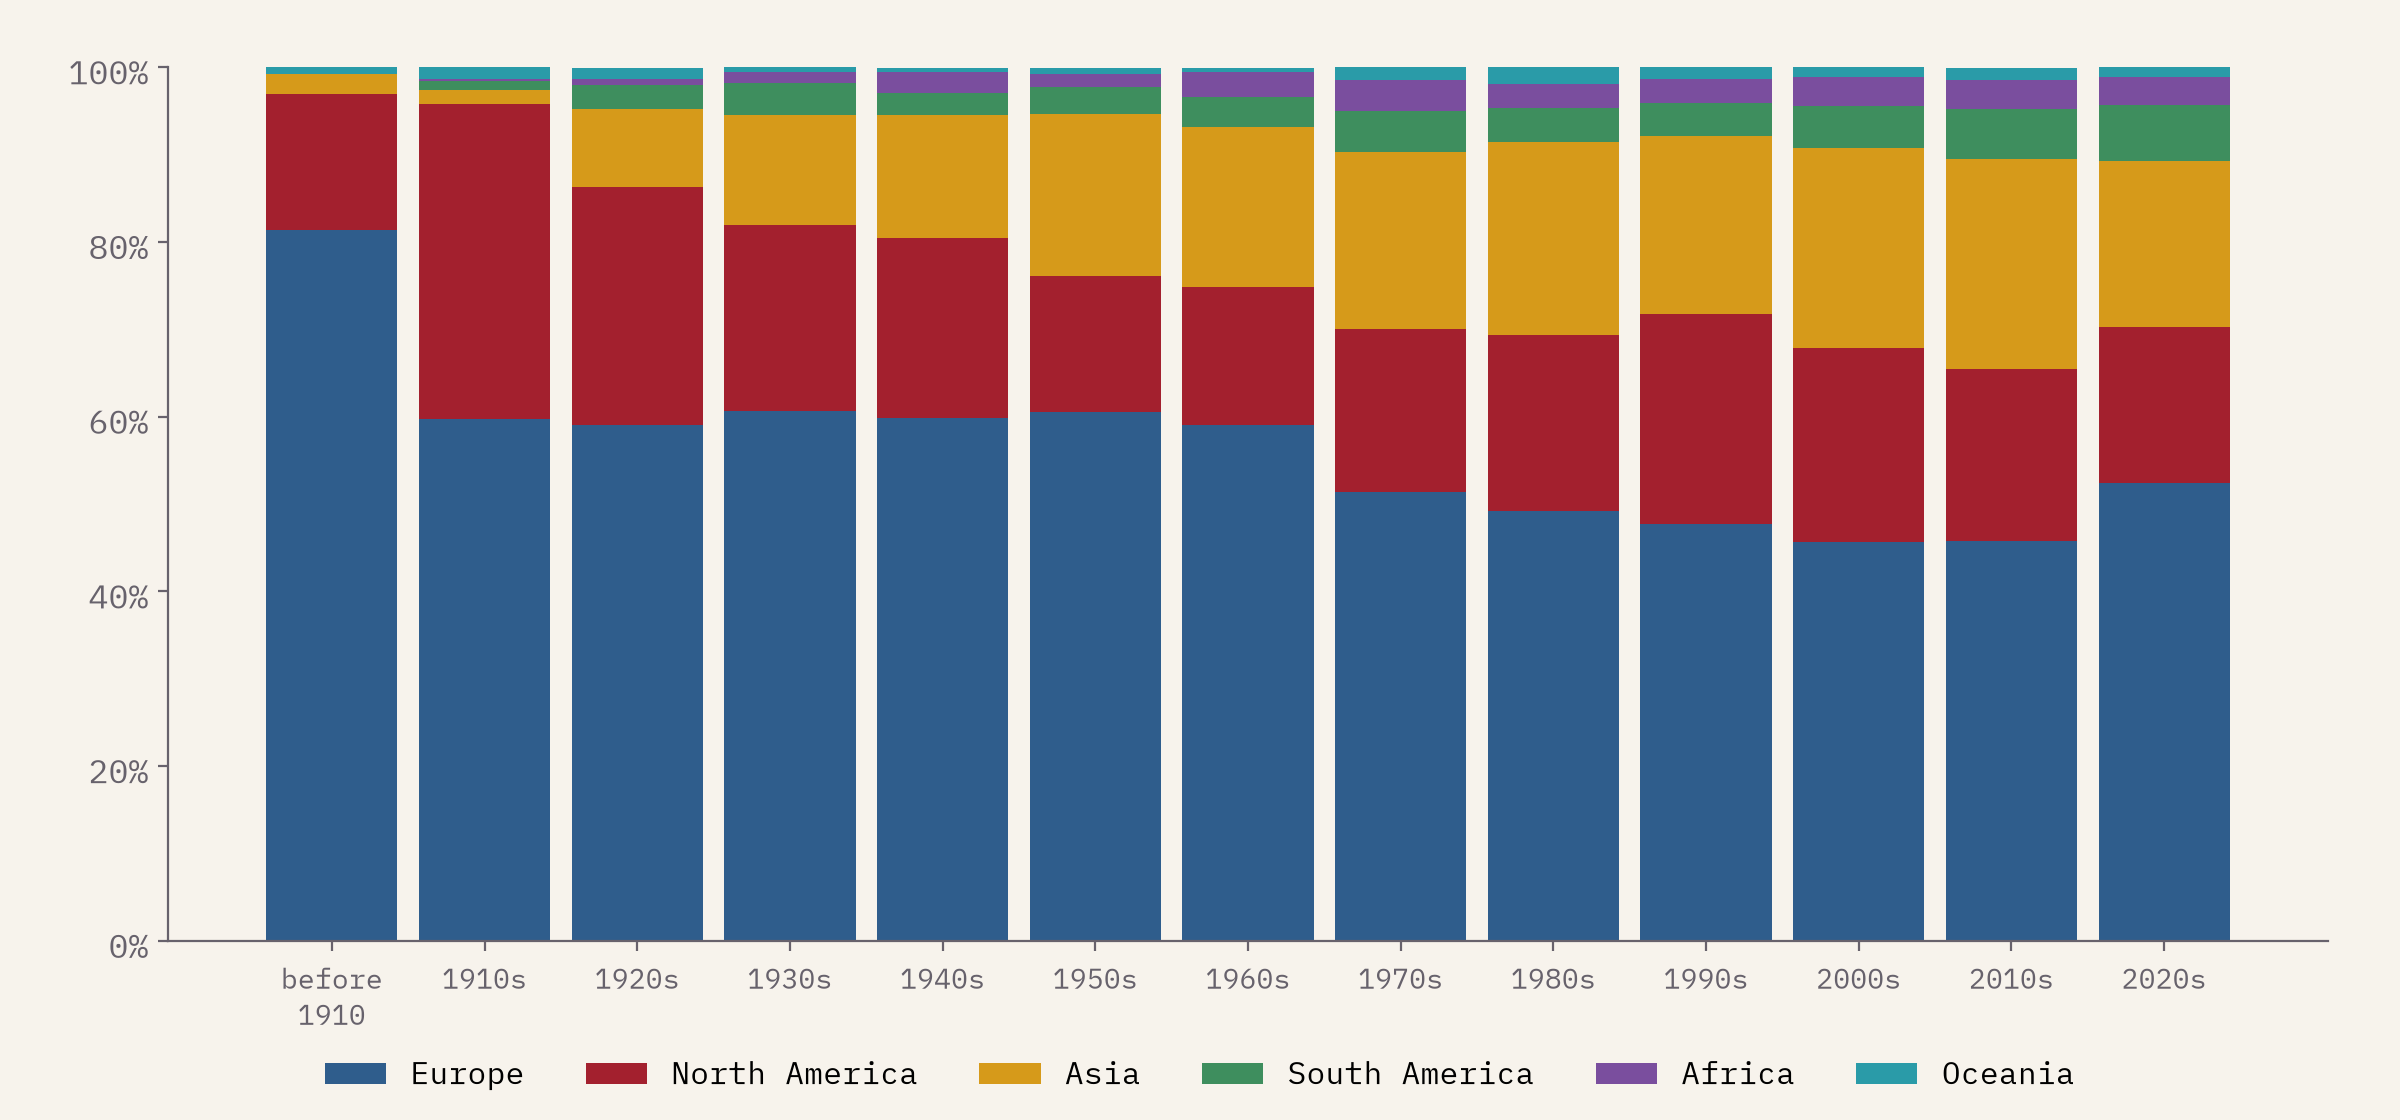
\includegraphics[width=\textwidth]{f_shift.png}
\caption{Continent of birth of directors, by the decade of their first dated film.}\label{fig:shift}\end{figure}

\begin{figure}[tbp]\centering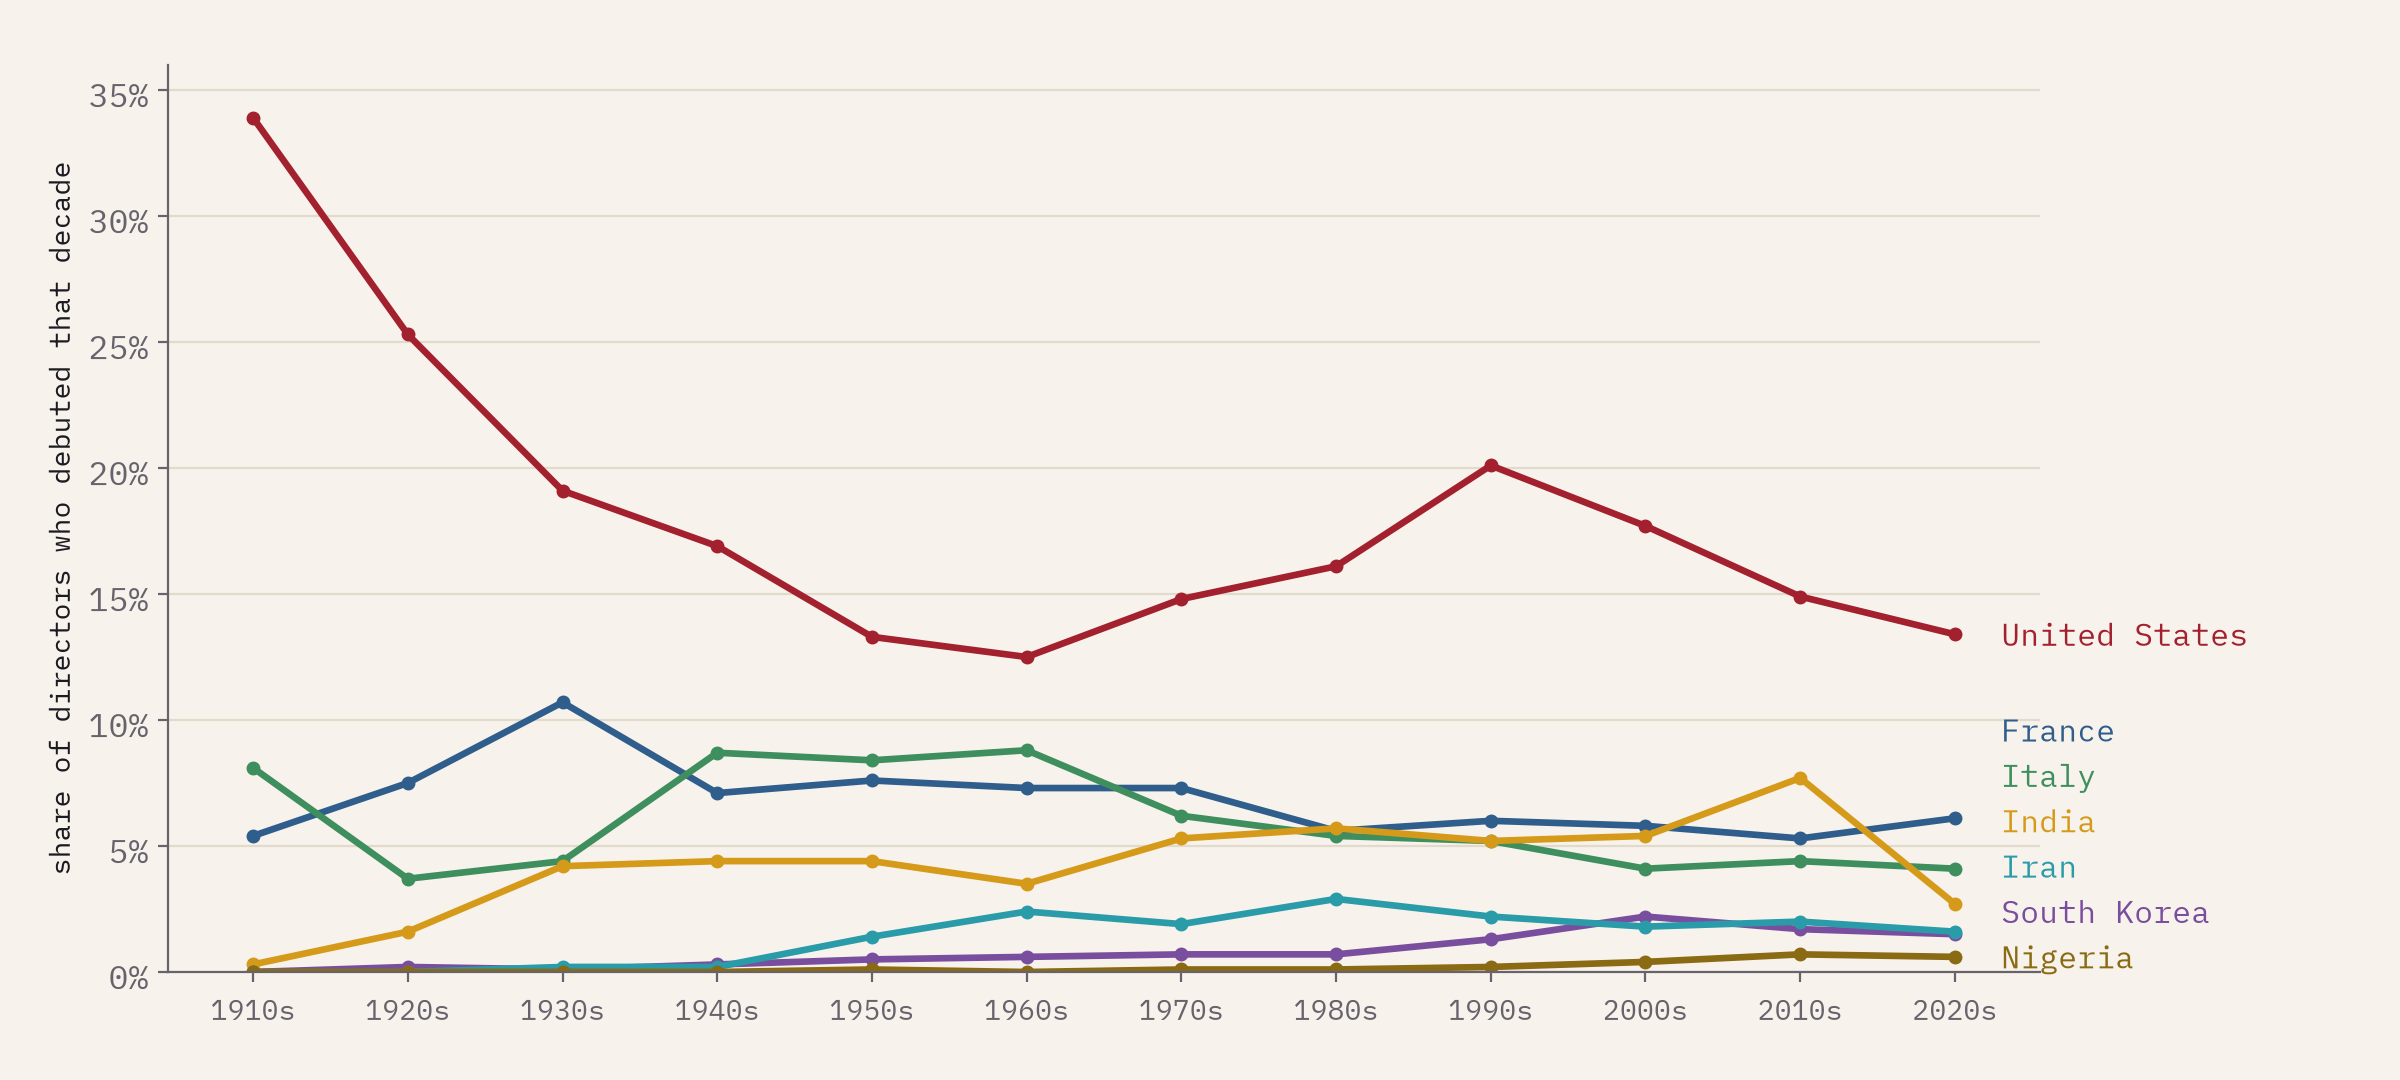
\includegraphics[width=\textwidth]{f_rise.png}
\caption{Share of each debut decade's directors born in selected countries.}\label{fig:rise}\end{figure}

\subsection{Directors who worked abroad}
15\% of 42,950 directors made their films mainly in a country other than the one they were born in. The share is remarkably stable, between about 14\% and 21\% in every decade from the 1910s. The largest flows (Figure~\ref{fig:flows}, Table~\ref{tab:flows}) are from the United Kingdom and Canada to the United States, from Austria, Poland and Switzerland to Germany, from China to Hong Kong and from Algeria to France. The countries that send the largest shares of their directors abroad are small neighbours of large film industries: Slovakia (37\%, mostly to the Czech Republic), Austria (36\%) and Switzerland, and also China (37\%, mostly to Hong Kong) and the United Kingdom (34\%). Of 8,455 directors whose films are mainly American, 20\% were born abroad, peaking at 24\% for those who debuted in the 1930s, in line with accounts of European directors in Hollywood \citep{petrie}.

\begin{figure}[tbp]\centering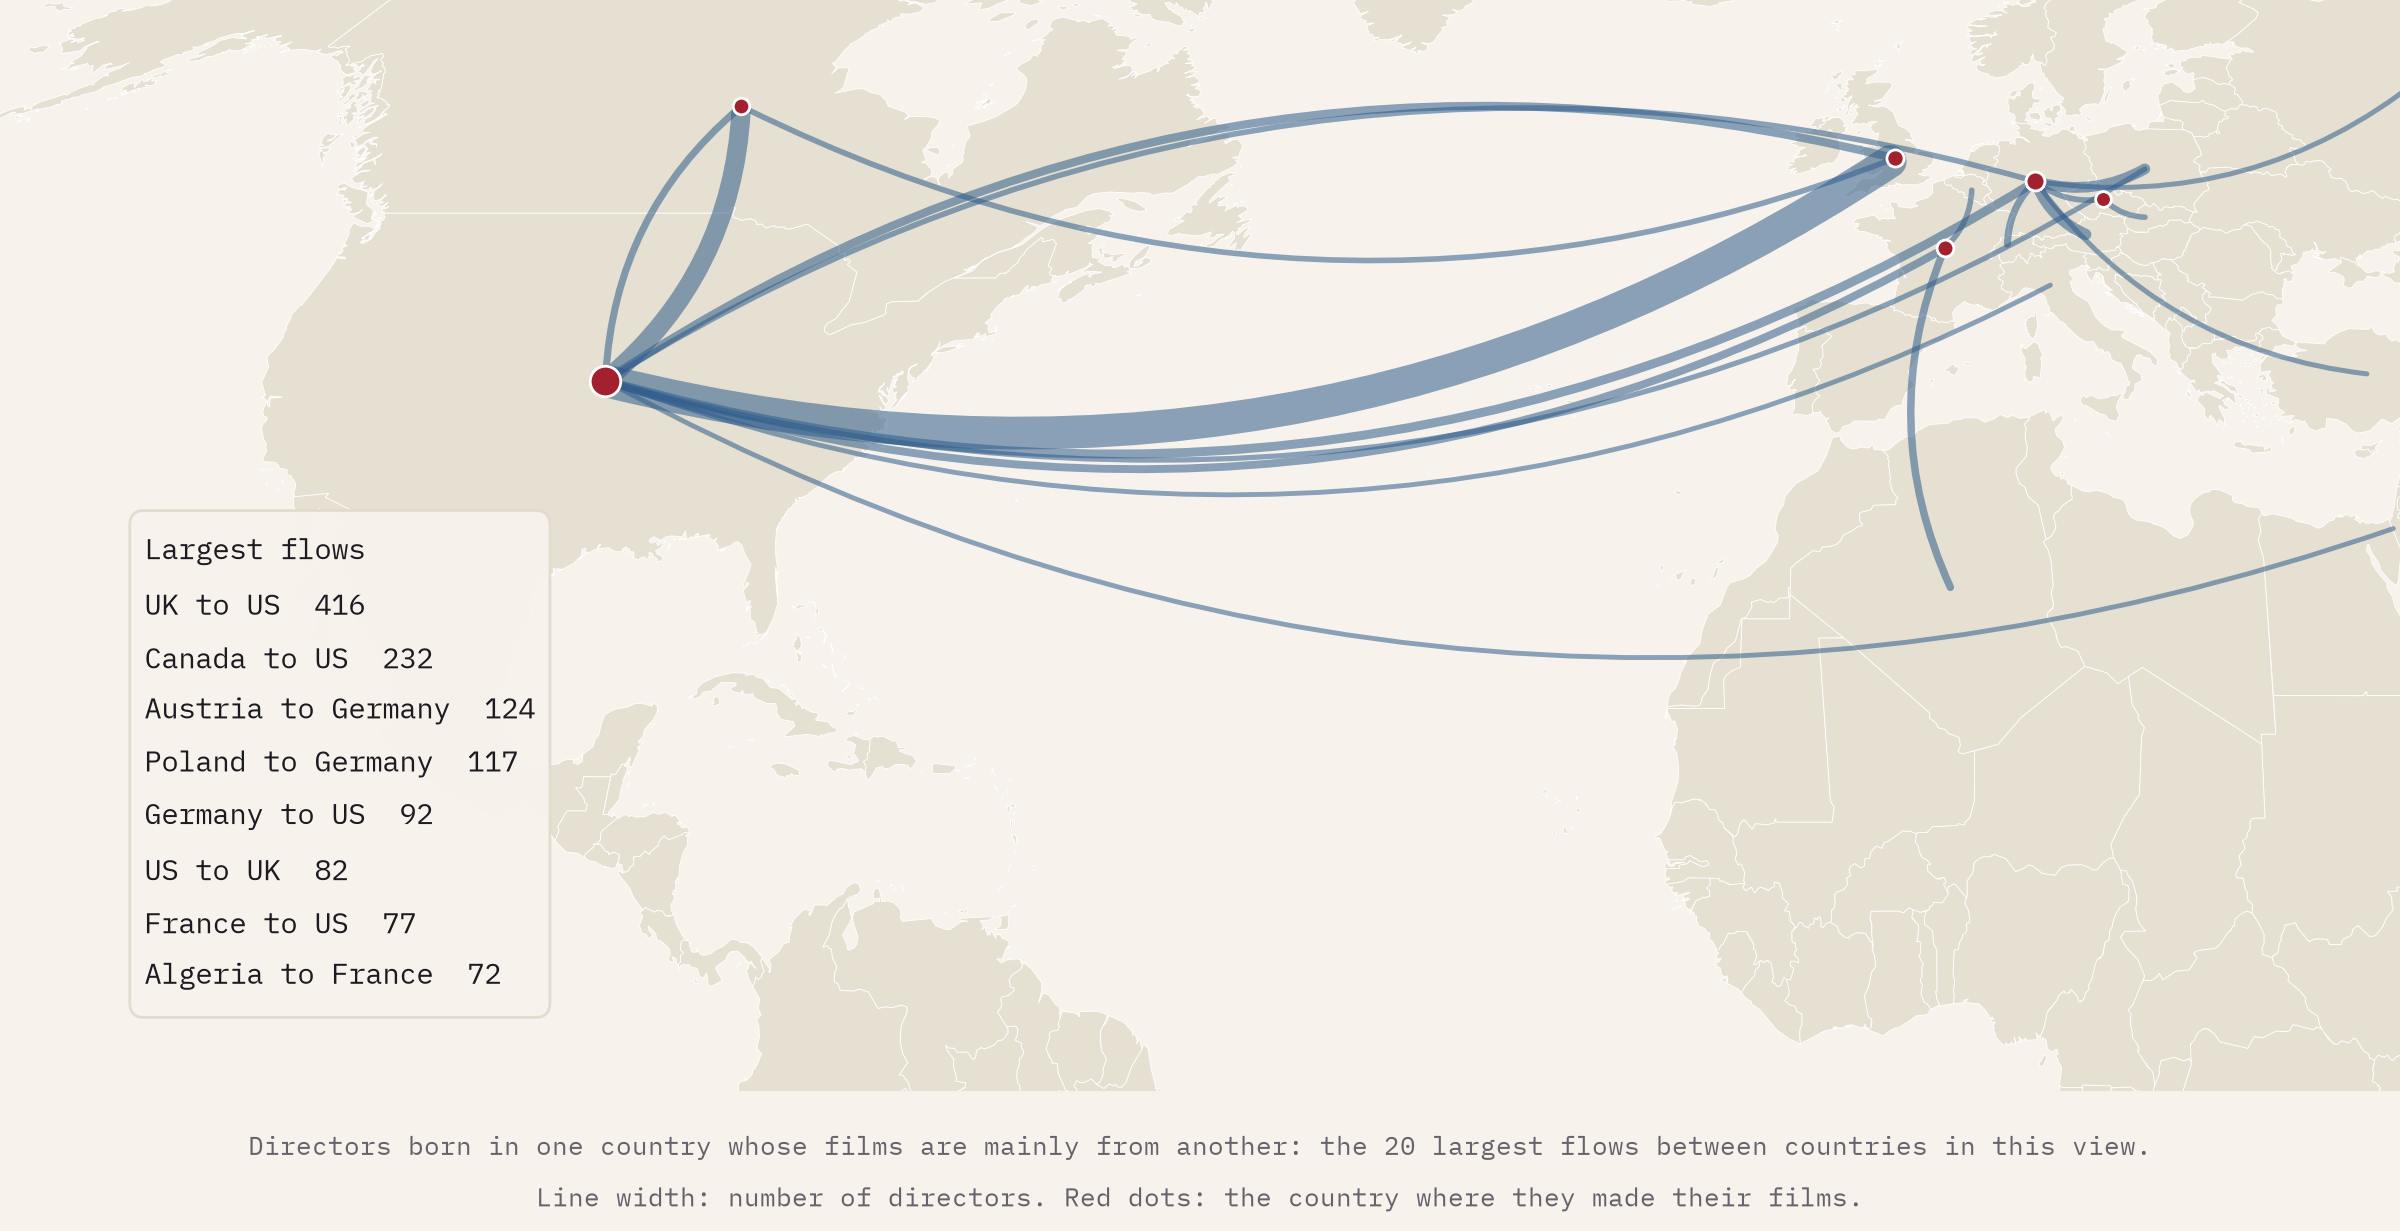
\includegraphics[width=\textwidth]{f_flows.png}
\caption{The largest flows of directors between countries around the North Atlantic, from birth country to main film country.}\label{fig:flows}\end{figure}

\begin{table}[tbp]\centering\small\caption{The largest flows from birth country to main film country.}\label{tab:flows}\begin{tabular}{llr}\toprule Born in & Films mainly from & Directors\\\midrule
United Kingdom & United States & 416\\
Canada & United States & 232\\
Austria & Germany & 124\\
Poland & Germany & 117\\
Germany & United States & 92\\
China & Hong Kong & 90\\
United States & United Kingdom & 82\\
France & United States & 77\\
Algeria & France & 72\\
United States & Canada & 66\\
Switzerland & Germany & 66\\
Australia & United States & 62\\
Czech Republic & Germany & 47\\
Slovakia & Czech Republic & 46\\
United States & Germany & 46\\
\bottomrule\end{tabular}\end{table}

\subsection{Women}
Women are 18.3\% of directors with a recorded gender. The share by debut decade (Figure~\ref{fig:women}, Table~\ref{tab:women}) starts with a handful of silent-era pioneers, Alice Guy-Blaché first among them, falls to 3.1\% in the 1920s and stays below 5\% until the 1970s, then rises to 9.1\% in the 1970s, 24.1\% in the 2010s and 32.0\% in the 2020s so far. Among notable directors the share is higher in recent decades (43.4\% in the 2020s), partly because recent notable `directors' include actors and musicians who directed one film. These figures sit well above industry counts of women directing the highest-grossing American films \citep{lauzen}, because Wikidata includes documentaries, short films and smaller national cinemas. By birth country, the highest shares are for directors born in Canada (26.7\%), Switzerland (26.1\%) and the Netherlands (24.5\%), and among the lowest are India (8.2\%) and Japan (8.5\%); these mix decades, so countries with mostly recent directors look better.

\begin{figure}[tbp]\centering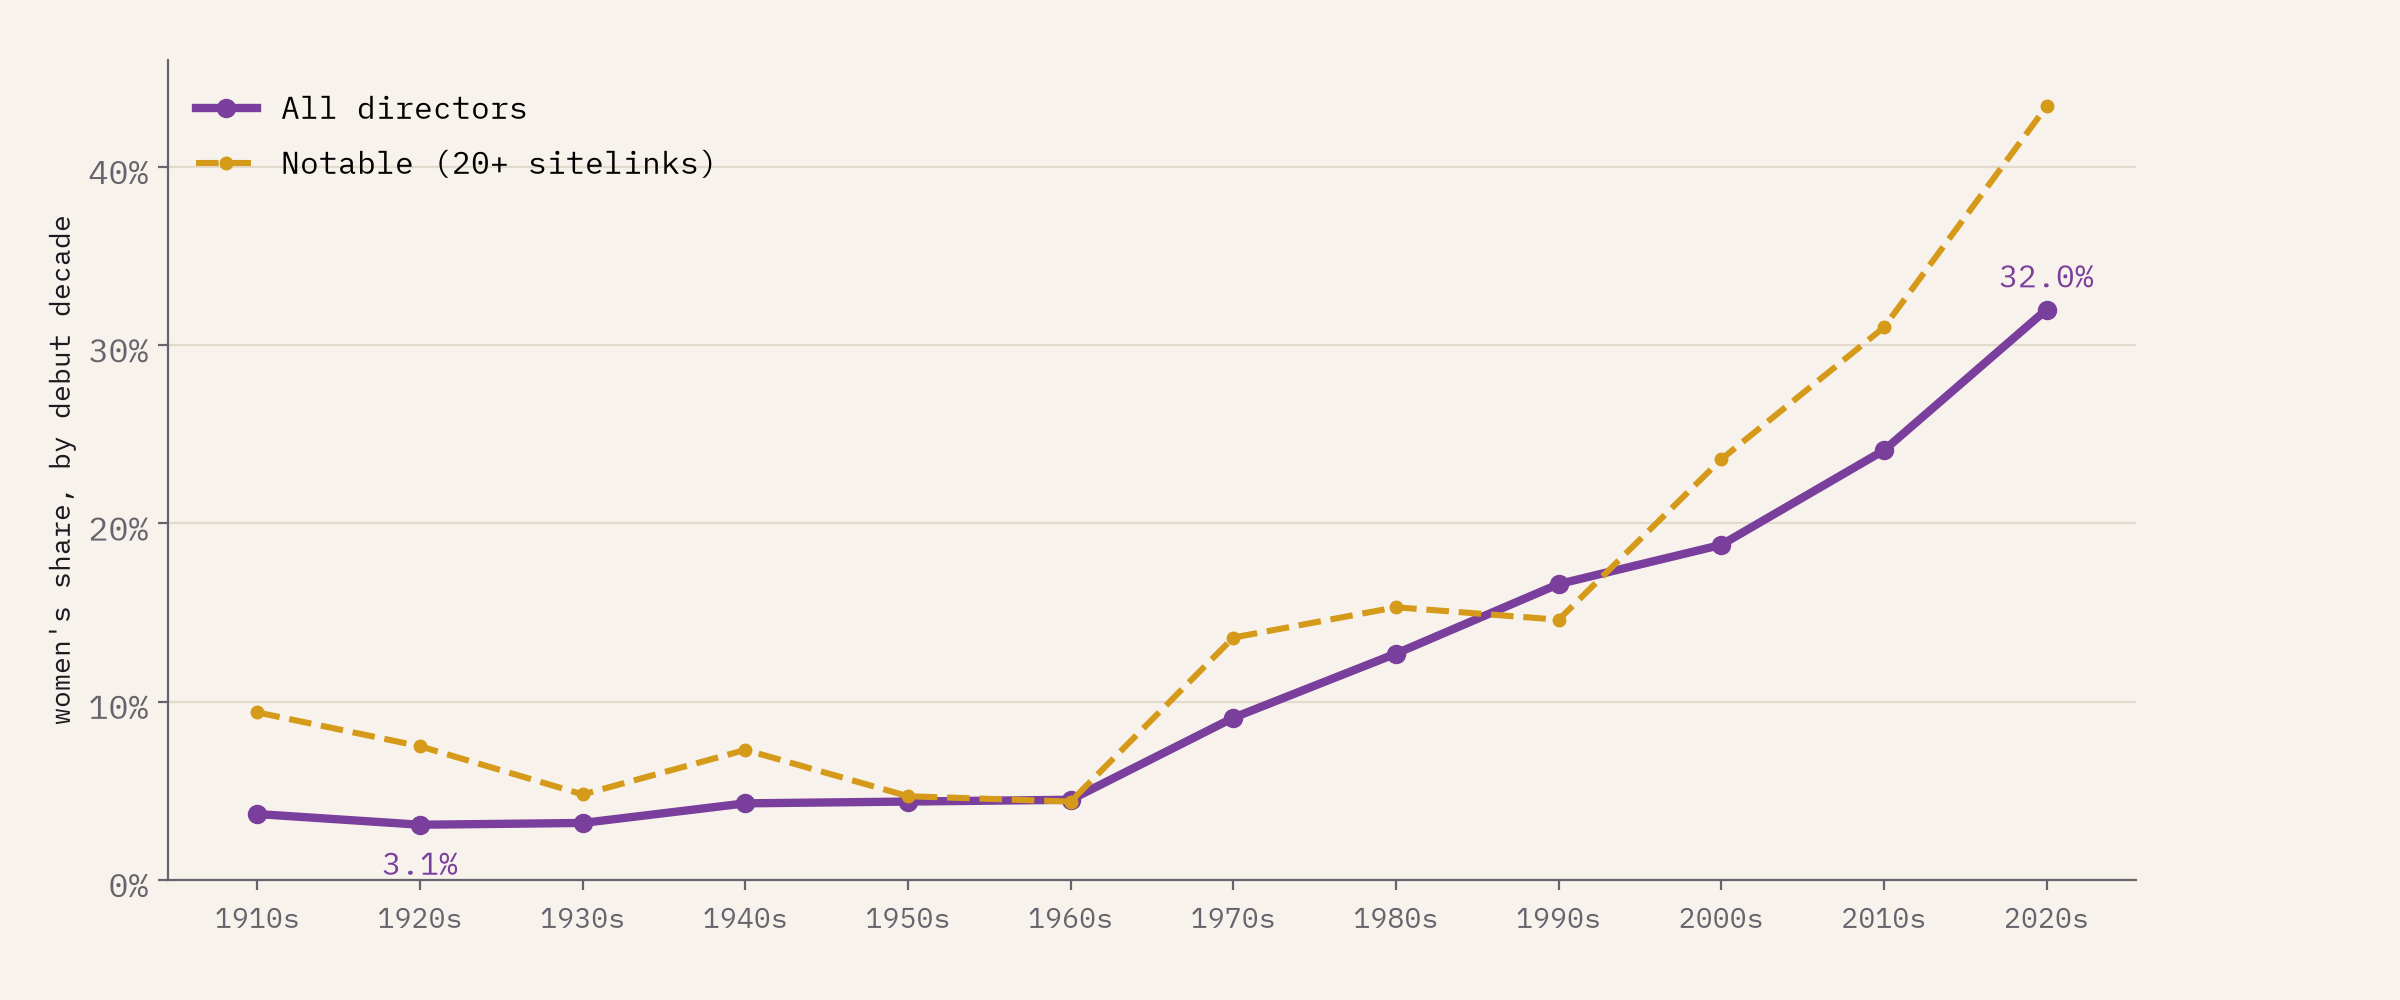
\includegraphics[width=\textwidth]{f_women.png}
\caption{Women's share of directors by debut decade, for all directors and notable directors.}\label{fig:women}\end{figure}

\begin{table}[tbp]\centering\small\caption{By debut decade: directors with a recorded gender, women, women's share among all and among notable directors, and the share of all directors with a birth country.}\label{tab:women}\begin{tabular}{lrrrrrr}\toprule Debut & With gender & Women & Share & Notable & Share & Birth country known\\\midrule
before 1910 & 151 & 2 & 1.3\% & 27 & 3.7\% & 81\%\\
1910s & 1,249 & 46 & 3.7\% & 127 & 9.4\% & 86\%\\
1920s & 1,273 & 40 & 3.1\% & 134 & 7.5\% & 82\%\\
1930s & 1,510 & 48 & 3.2\% & 145 & 4.8\% & 83\%\\
1940s & 1,324 & 57 & 4.3\% & 137 & 7.3\% & 80\%\\
1950s & 2,275 & 100 & 4.4\% & 233 & 4.7\% & 79\%\\
1960s & 3,518 & 159 & 4.5\% & 319 & 4.4\% & 79\%\\
1970s & 4,503 & 411 & 9.1\% & 346 & 13.6\% & 70\%\\
1980s & 5,552 & 706 & 12.7\% & 367 & 15.3\% & 63\%\\
1990s & 6,880 & 1,139 & 16.6\% & 522 & 14.6\% & 60\%\\
2000s & 13,695 & 2,571 & 18.8\% & 669 & 23.6\% & 55\%\\
2010s & 18,828 & 4,535 & 24.1\% & 520 & 31.0\% & 43\%\\
2020s & 6,426 & 2,056 & 32.0\% & 196 & 43.4\% & 42\%\\
\bottomrule\end{tabular}\end{table}

\subsection{Prolific directors}
Half of all directors have 1 film in Wikidata, and 53\% exactly one; 353 have fifty or more. The most prolific are silent and studio-era directors of short and series films: Louis Feuillade (254 films), Lau Lauritzen Sr. (217), Sam Newfield (203), William Beaudine (188) and Richard Thorpe (179). The most prolific woman is Alice Guy-Blaché (75).

\subsection{Coverage}
Birthplace coverage is the main limitation (Figure~\ref{fig:cov}). Notable directors almost always have a birthplace (99.5\%), directors with at most one sitelink only 25\%. By main film country, coverage ranges from over 80\% for Hungary, Russia, Italy and Iran to about a third for Canada, Denmark and Nigeria (33\% of 372 directors). The share of directors with a birth country also falls for recent debut decades, from 79\% for the 1950s to 43\% for the 2010s, as bulk imports of recent films add names without biographies.

\begin{figure}[tbp]\centering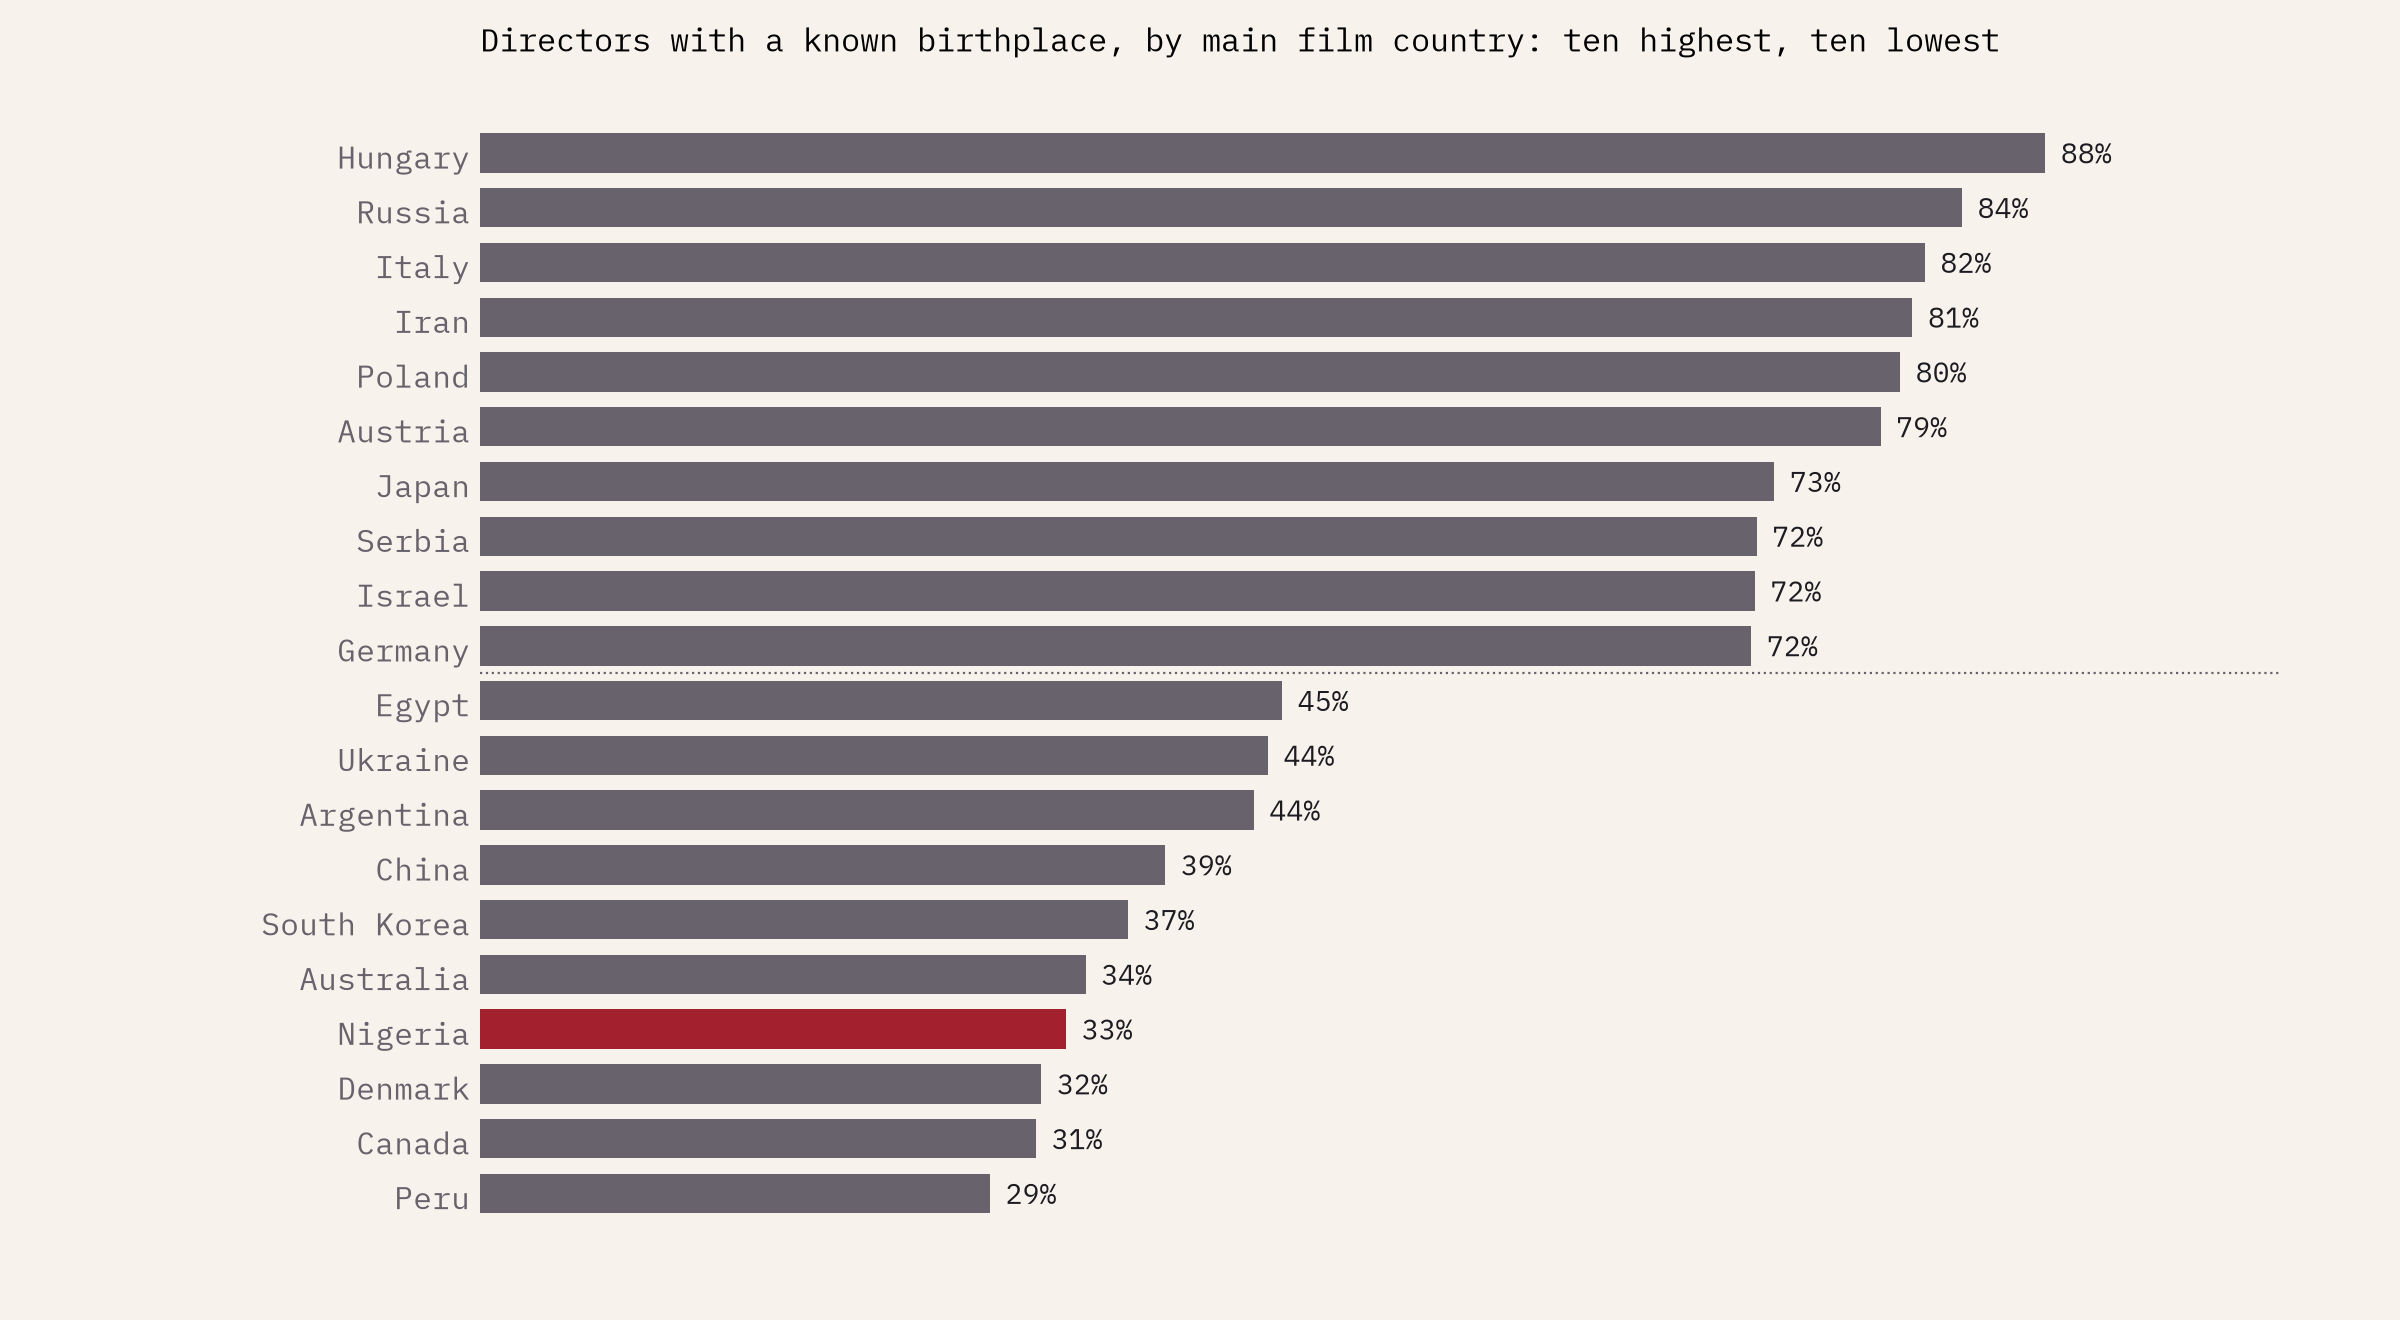
\includegraphics[width=\textwidth]{f_coverage.png}
\caption{Share of directors with a known birthplace, by main film country (countries with 350 or more directors).}\label{fig:cov}\end{figure}

\section{Discussion}
The open record reproduces several familiar features of film history: the early dominance of France, the United States and Germany; the long importance of European-born directors in Hollywood; the growth of Indian, Korean and Iranian cinema; and the slow, late rise of women behind the camera. It also adds texture that national histories rarely show, such as the concentration of directors in a few great cities and the steady one-in-seven share of directors who worked mainly in another country.

Every one of these findings is shaped by coverage. A country's number of directors in Wikidata depends on whether its film database has been imported, and whether the import included birthplaces; Prague's and Copenhagen's high per-head rates and Nigeria's near absence are in large part facts about the record. Sitelinks, used here to define notable directors, measure attention on Wikipedia and favour celebrities who directed a single film. The safest comparisons are within the data over time, such as women's share by decade, and even these are affected by which recent films have been added.

\section{Limitations}
First, Wikidata is incomplete and uneven, and 55\% of directors have a birthplace. Second, the population is defined by Wikidata's film class and director property, which include short films and documentaries and exclude television, and the people include non-professional directors. Third, birth countries use present-day borders. Fourth, the debut year is the earliest dated film in Wikidata, which may be later than a director's real debut. Fifth, a main film country splits co-productions equally and treats former states through a hand-made table of successors. Sixth, gender is as recorded, mostly binary, and missing for 10\% of directors. Seventh, city areas use a fixed 30 km radius and present-day populations. Finally, all counts are for one retrieval in 2026.

\section{Conclusion}
Two open queries are enough to map where tens of thousands of film directors were born, how that geography moved from Europe and North America towards Asia, which directors left home to make films, and how long it took for women to appear in numbers. The same data show clearly where the record is thin. The atlas lets readers explore both.

\section*{Data and code availability}
The interactive atlas is at \url{https://maps.tristanhotham.com/director-birthplaces/}. Data and code are at \url{https://github.com/Tristan-Hotham/director-birthplaces} and archived with this paper at https://doi.org/10.5281/zenodo.23847840. Derived data are released under CC BY 4.0 and code under the MIT licence.

\section*{AI statement}
I wrote the text, with drafting and editing assistance from Claude (Anthropic), which also helped prepare the analysis code. I reviewed and checked all text and results.

\begin{thebibliography}{9}
\bibitem[Bast and Buchhold(2017)]{qlever} Bast, H. and Buchhold, B. (2017) QLever: a query engine for efficient SPARQL+text search. \emph{Proceedings of the 2017 ACM Conference on Information and Knowledge Management}, 647 to 656. \url{https://qlever.cs.uni-freiburg.de/}
\bibitem[Haynes(2016)]{haynes} Haynes, J. (2016) \emph{Nollywood: The Creation of Nigerian Film Genres}. Chicago: University of Chicago Press.
\bibitem[Lauzen(2024)]{lauzen} Lauzen, M. M. (2024) \emph{The Celluloid Ceiling}. San Diego: Center for the Study of Women in Television and Film, San Diego State University.
\bibitem[Natural Earth(2026)]{naturalearth} Natural Earth (2026) Admin 0 countries and populated places. Public domain. \url{https://www.naturalearthdata.com/}
\bibitem[Petrie(2002)]{petrie} Petrie, G. (2002) \emph{Hollywood Destinies: European Directors in America, 1922 to 1931}. Revised edition. Detroit: Wayne State University Press.
\bibitem[Schich et al.(2014)]{schich} Schich, M., Song, C., Ahn, Y.-Y., Mirsky, A., Martino, M., Barab\'asi, A.-L. and Helbing, D. (2014) A network framework of cultural history. \emph{Science}, 345(6196), 558 to 562.
\bibitem[Vrandečić and Krötzsch(2014)]{wikidata} Vrandečić, D. and Krötzsch, M. (2014) Wikidata: a free collaborative knowledgebase. \emph{Communications of the ACM}, 57(10), 78 to 85.
\bibitem[Wagner et al.(2016)]{wagner} Wagner, C., Graells-Garrido, E., Garcia, D. and Menczer, F. (2016) Women through the glass ceiling: gender asymmetries in Wikipedia. \emph{EPJ Data Science}, 5, 5.
\end{thebibliography}
\end{document}
